\documentclass[11pt]{article}
\usepackage{fullpage}
\usepackage{graphicx}
\usepackage{url}
\usepackage{listings}
\usepackage{amsmath}

\lstset{
    basicstyle=\ttfamily\small,
    breaklines=true,
    frame=single
}

\setlength{\parindent}{0pt}
\setlength{\parskip}{8pt}

\title{CS140 - Assignment 7\\\small{\emph{Due: Sunday, Mar. 24 at 11:59pm}}}
\author{}
\date{}

\begin{document}

\maketitle

\begin{center}
% \includegraphics[scale=0.4]{figures/big_picture.jpg}
\footnotesize{http://www.smbc-comics.com/index.php?db=comics\&id=2217}
\end{center}

\newpage

\noindent For this assignment, you may (and are encouraged to) work with a partner.

\begin{enumerate}

\item \textbf{[5 points]} Huffman codes

Suppose the symbols $a$, $b$, $c$, $d$, $e$ occur with frequencies 30, 20, 15, 40, 60 respectively, in a file.

\begin{enumerate}

\item What is the Huffman encoding of the alphabet?  Note, follow the algorithm in class, where the smallest value is the left branch and the next smallest is the right branch.  For encoding, the left branch will be 0 and the right branch 1.

\begin{figure}
    \centering
    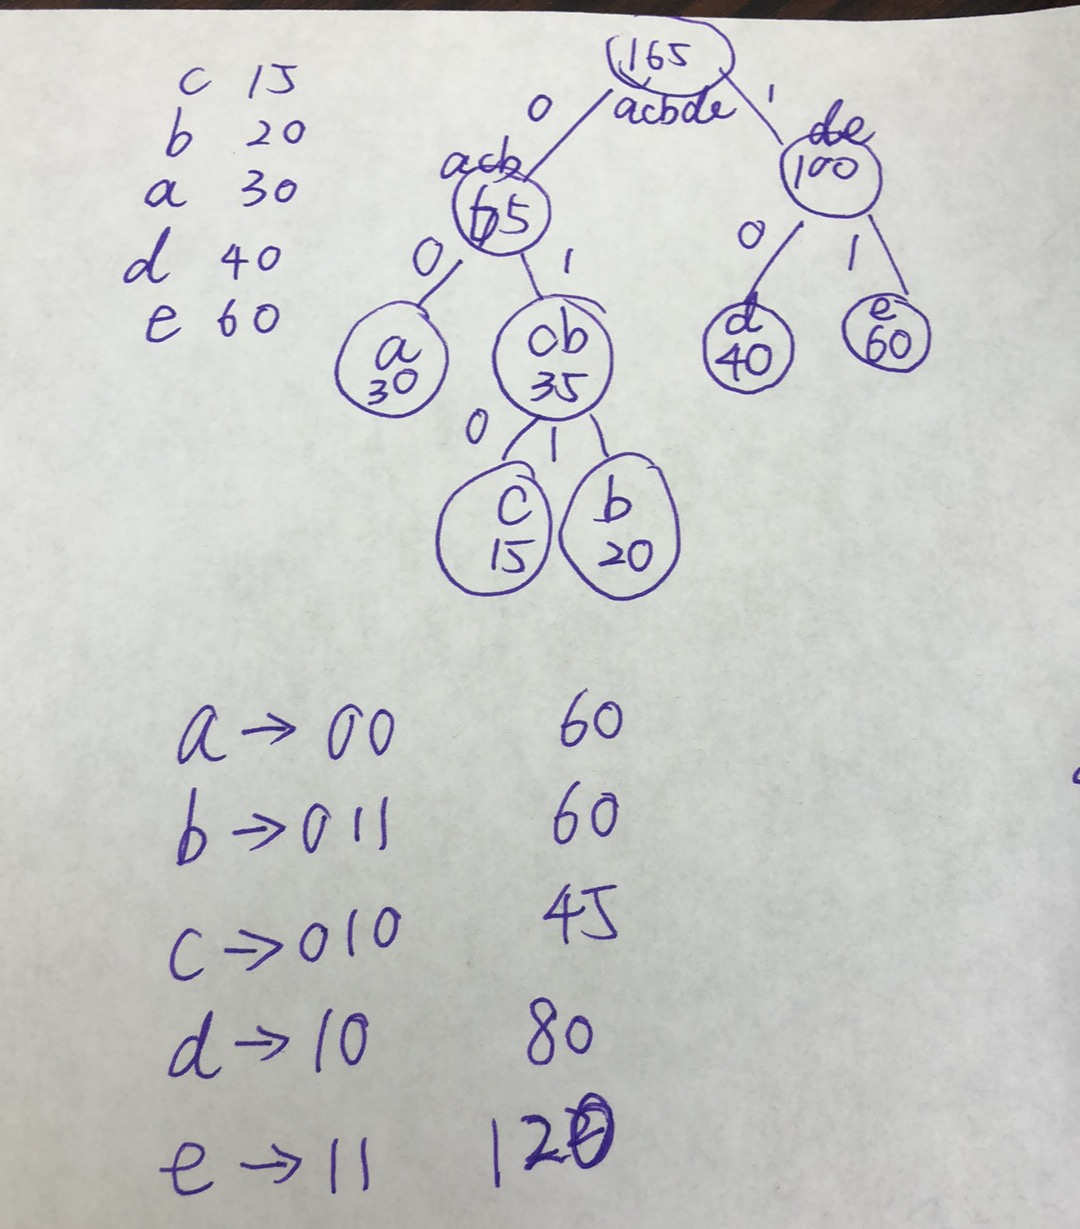
\includegraphics[width=0.5\linewidth]{image.png}
    \caption{Enter Caption}
    \label{fig:enter-label}
\end{figure}
\item If this encoding is applied to the file, what is the length of the encoded file in bits?
 365    

\end{enumerate}
\end{enumerate}

\section*{Greedy or DP}

One of the problems below can be solved more efficiently using a greedy approach and the other cannot (i.e. you must use dynamic programming).  For each problem clearly describe your algorithm and state the run-time.  For the dynamic programming problem, make sure to describe the table and how it is filled in.  For the greedy problem, argue (a formal proof isn't necessary) that your solution is optimal.

\begin{enumerate}

\setcounter{enumi}{1}

\item \textbf{[10 points]} You're going on a road trip with friends.  Unfortunately, your headlights are broken, so you can only drive in the daytime.  Therefore, on any given day you can drive no more than $d$ miles.  You have a map with $n$ different hotels and the distances from your start point to each hotel $x_1 < x_2 < ... < x_n$.  Your final destination is the last hotel.  Describe an algorithm that determines which hotels you should stay in if you want to minimize the number of days it takes you to get to your destination.

\textbf{Answer}:

The most efficient solution for this problem is a greedy algorithm. Our strategy hinges on the idea of maximizing the distance traveled each day, up to the limit of $d$ miles, by selecting the furthest hotel within this range. This means, starting from the initial location, we aim to stay at the hotel that is the furthest away, yet does not surpass the daily mileage cap of $d$ miles. This process is repeated daily until we arrive at the final destination.

By consistently opting for the hotel that allows us to cover the greatest distance without going over $d$ miles, we minimize the total number of travel days required to reach our endpoint, thereby avoiding unnecessary stops.

The runtime is $O(n)$ where $n$ is the number of hotels since you might have to check each hotel once to decide whether or not you're able to go to the next hotel (since we cannot exceed $d$ miles a day).

\item \textbf{[10 points]} Same setup as above, however, you also want to do some sightseeing along the way.  To make sure you don't spend too little or too much time in any one place, you decide to add a penalty for having too much free time.  If you travel $x$ miles in a day, then the penalty for that day is $(d - x)^2$.  Describe an algorithm that determines the hotel sequence that minimizes the total penalty, that is the sum of the daily penalties over all travel days.

Let's outline a dynamic programming (DP) approach using an array as our DP table. In this array, each index corresponds to a hotel number, counting from the start point to the destination, with an additional initial index serving as our "base case" for the dynamic programming calculation. The values stored at these indices represent the least penalty incurred to reach each hotel, either directly from the start or via any preceding hotels. The daily penalty is calculated as $(d - (x_{\text{curr}} - x_{\text{prev}}))^2$.

To determine the minimum penalty for each hotel, we consider reaching it from the start or any earlier hotel, using the formula:

\begin{lstlisting}[language=Python]
DPTable[3] = min(DPTable[3], DP[i] + (d - (x[3] - x[i]))^2)
\end{lstlisting}

Here, $DP[i]$ represents the minimum penalty for reaching a previously considered hotel, and we iterate through each prior hotel as long as the travel distance $(x[3] - x[i]) \leq d$ does not exceed the daily limit $d$. Each $DP[i]$ entry captures the lowest penalty necessary to arrive at hotel $i$.

Starting from the second hotel, we iteratively compute the minimum penalty for reaching each hotel, taking into account all feasible preceding hotels within the daily mileage restriction. We then update each $DP[i]$ based on the calculated penalties from all eligible preceding hotels.

The computational complexity is $O(n^2)$ since, for each hotel, the penalty calculations involve comparisons with potentially all preceding hotels, under the constraint of $d$ miles per day. This process entails making $n$ comparisons for each of the $n$ hotels. To trace the optimal path of hotel stays, one could maintain a record of the indices in the array where stops are made, particularly when the constraint of $d$ miles per day is breached.

The optimal total penalty for the entire trip is then located in $DP[n]$, with $n$ being the index of the final destination hotel.

\end{enumerate}

\section*{More fun}

\begin{enumerate}

\setcounter{enumi}{3}


\item \textbf{[10 points]} Given a set of points ${x_1, x_2, ..., x_n}$ on the real line, describe a greedy algorithm that determines the smallest set of unit-length (i.e., length=1) closed intervals that contains all of the given points.  State the worst case running time and prove that your algorithm is correct.  You do not need write pseudo-code, but make your description clear.

Sort all the points then imagine a line and we go from left to right, we need to find the first point and use a interval to cover it( make sure start the interval exactly at the point) and then we ignore the points is being covered by this interval, we go to the next first point which is not being covered and put another interval to cover it ( make sure start the interval exactly at the point) and then we ignore the points is being covered by this interval, ... we keep doing this until we reach to the last point.  The worst case running time would be O(nlogn), a case where all the points is far ahead(more than interval) from each other so we need one interval for each point, so we need to go through all the points.  Using stays ahead principle it shows that the algorithm  always covers as many points as possible since the greedy choice of placing an interval starting exactly at the earliest uncovered point covers as many points as possible up to that point. By the nature of the sorted points, no interval can start later and still cover more points. Therefore, this greedy choice always leads to an optimal solution for the subproblem up to that point, and by extension, the entire set of points.

\item \textbf{[7 points]} Hashtable review

\begin{enumerate}

\item \textbf{[3 points]} Show the result of inserting 5, 28, 19, 15, 20, 10, 33, 12, 17 into a hashtable with collision resolution by chaining.  The table should have 9 slots and use $h(k) = k$ mod $9$ for the hash function.

\begin{enumerate}
    \item Slot 0: 
    \item Slot 1: 10 => 19 => 28
    \item Slot 2: 20
    \item Slot 3: 12
    \item Slot 4: 
    \item Slot 5: 5
    \item Slot 6: 33=>15
    \item Slot 7: 
    \item Slot 8: 17
\end{enumerate}


\item \textbf{[3 points]} Show the result of inserting the first 6 of these into another hashtable using open addressing and linear probing.

Slot 0: 
Slot 1: 28
Slot 2: 19
Slot 3: 20
Slot 4: 10
Slot 5: 5
Slot 6: 15
Slot 7: 
Slot 8: 

\item \textbf{[1 points]} For the these insertions, what was the largest number of collisions you had before finding an open slot and what key was it?
3 for 10


\end{enumerate}

\end{enumerate}

\end{document}
